\section{Results}\label{sec:hmmResults}

The first result to consider is the number of events observed in the invariant-mass range $\muu\in[120,130]$~GeV.
This region contains the majority of the VH signal and is the primary focus of this analysis.
The observed yields are provided in Table \ref{tab:hmmResultNdat} along with the number of expected background events in the same region.
The first thing to stand out is the slight excesses of observed events over the expected events in the inclusive 4-lepton and 3-lepton categories.
These excesses are preserved in the post-cut exclusive categories.
The significances of these excesses will be given later, but it is interesting to note that the subsequent measurement by CMS found a similar excess in leptonic VH events. 

Figures \ref{fig:hmmPrecutFits} and \ref{fig:hmmPostcutFits} show the invariant mass distributions of the data.
Both the signal+background (Equation \ref{eqn:hmmSbFunc}) and background-only (Equation \ref{eqn:hmmBkgFunc}) models are fit to the data  and shown as well.
The excesses in the region near the Higgs mass lead the signal strength measured by the S+B models to be positive.

\begin{table}[htp]
\begin{center}
\begin{tabular}{l r r r r r}\toprule
Category               & Data    & Background \\
\midrule
4-Lepton               & 51      & 47.3$\pm$2.7 \\
3-Lepton               & 437     & 414.2$\pm$18.6 \\
\midrule
4-Lepton High-Purity   & 34      & 22.8$\pm$1.4 \\
3-Lepton High-Purity   & 41      & 34.8$\pm$2.2 \\
3-Lepton Middle-Purity & 358     & 341.3$\pm$15.8 \\
\bottomrule\end{tabular}\\
\caption{
Yields of data and expected background counted in invariant-mass range $\muu\in[120,130]$~GeV.
The uncertainties on the background estimate are described in Section \ref{sec:hmmBkgUncert}.
}
\label{tab:hmmResultNdat}
\end{center}
\end{table}


\begin{figure}[h!]
\captionsetup[subfigure]{position=b}
\centering
\subfloat[][]{{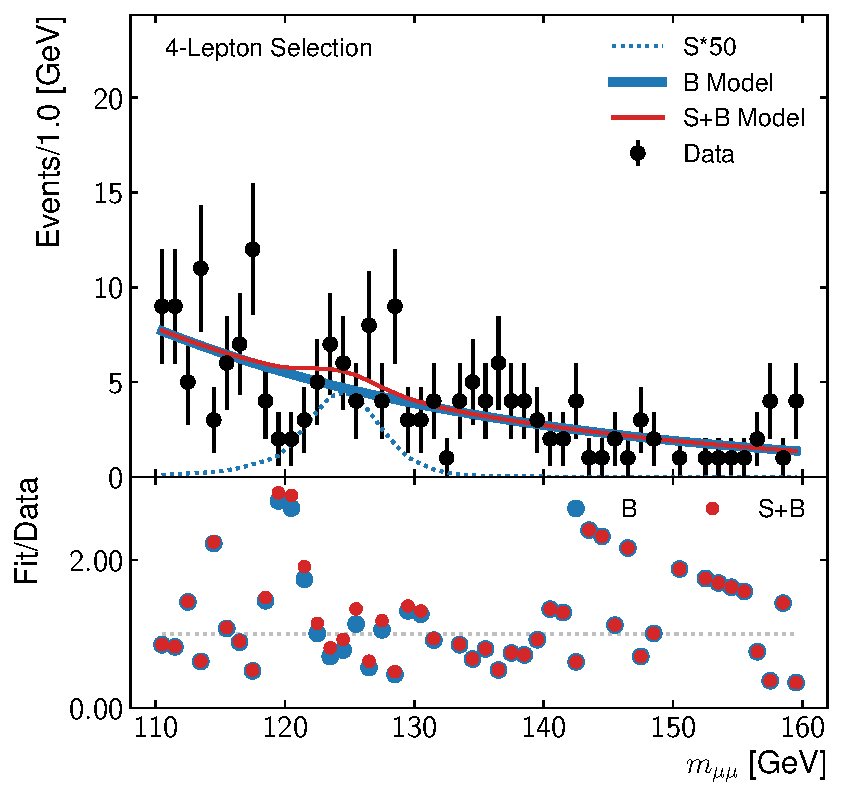
\includegraphics[width=0.5\textwidth]{figures/hmm/fitData/ratio-4lep-dat.pdf}}}
\subfloat[][]{{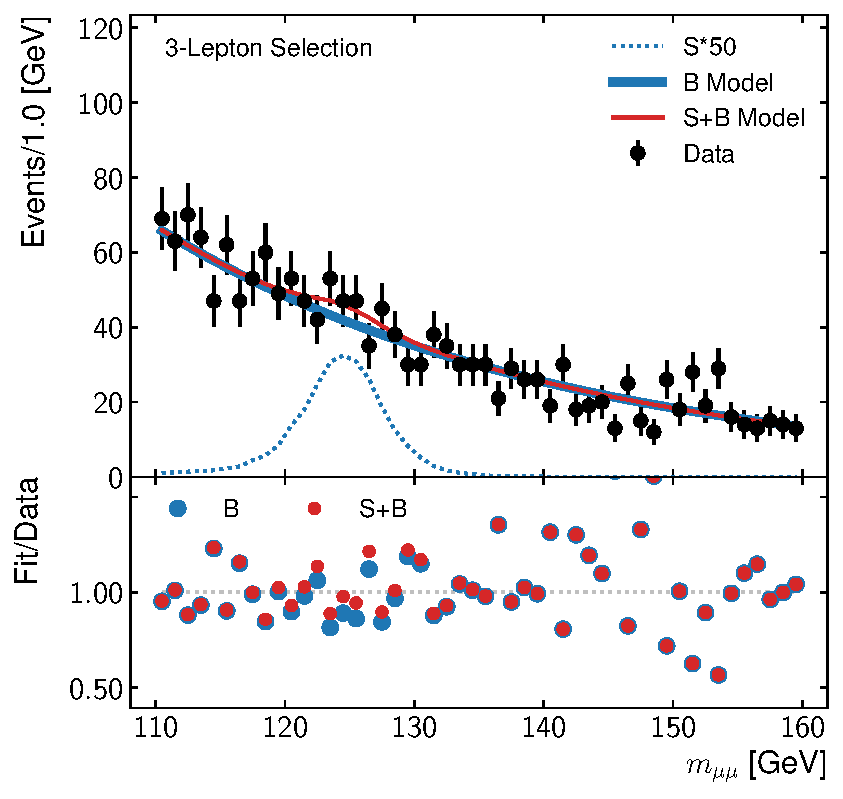
\includegraphics[width=0.5\textwidth]{figures/hmm/fitData/ratio-3lep-dat.pdf}}}
\caption{Fits of the S+B and B-only models to the data observed in the inclusive 4-lepton (a) and 3-lepton (b) categories.}
\label{fig:hmmPrecutFits}
\end{figure}

\begin{figure}[h!]
\captionsetup[subfigure]{position=b}
\centering
\subfloat[][]{{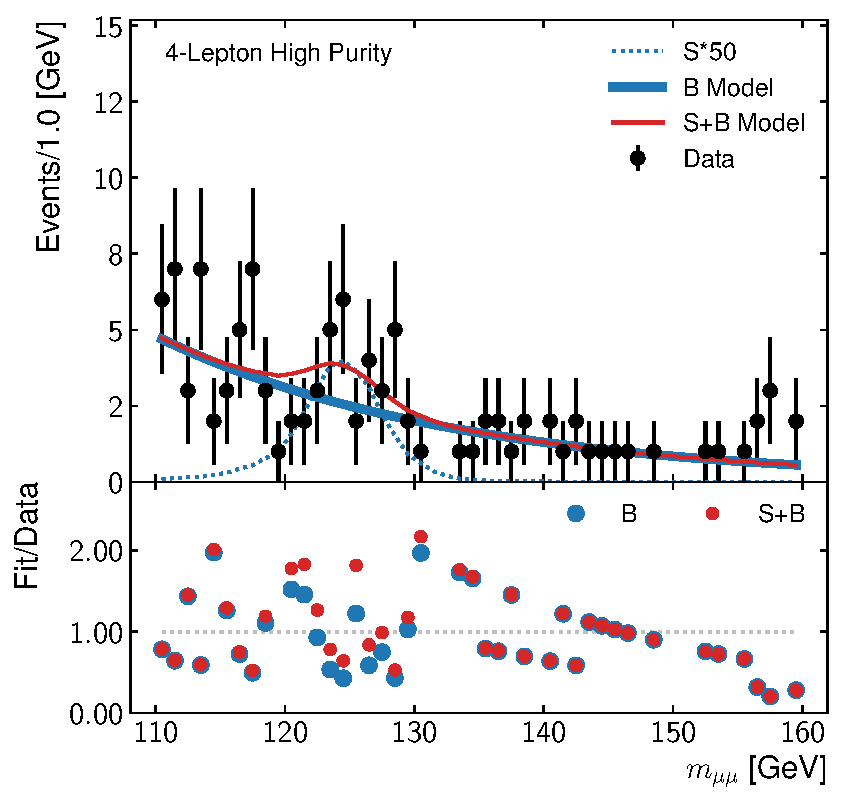
\includegraphics[width=0.5\textwidth]{figures/hmm/fitData/ratio-4lep0-dat.pdf}}}
\subfloat[][]{{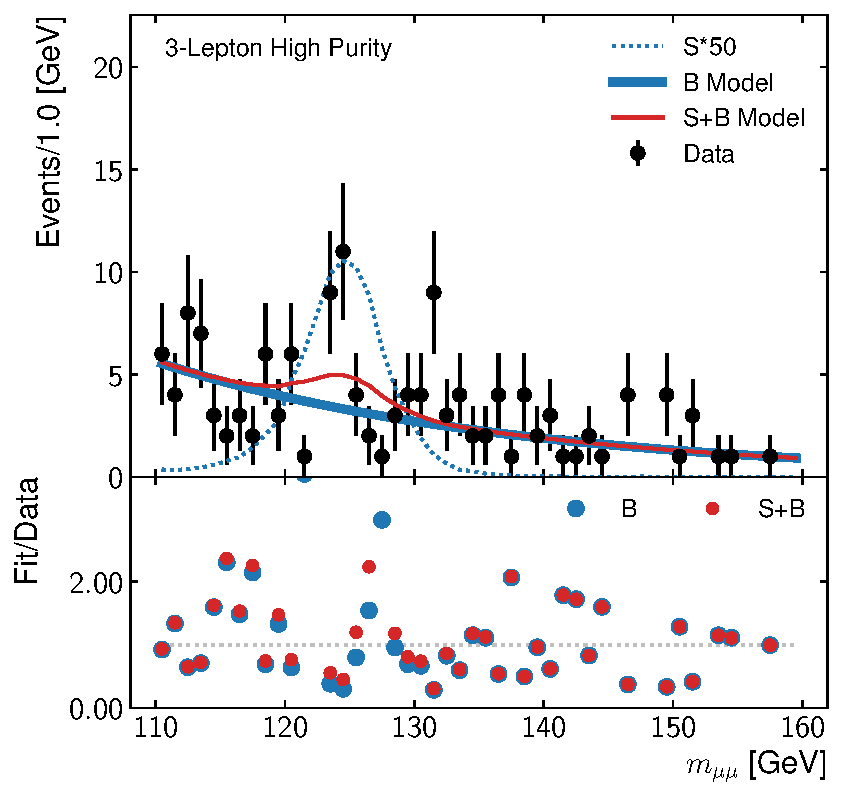
\includegraphics[width=0.5\textwidth]{figures/hmm/fitData/ratio-3lep0-dat.pdf}}} \\
\subfloat[][]{{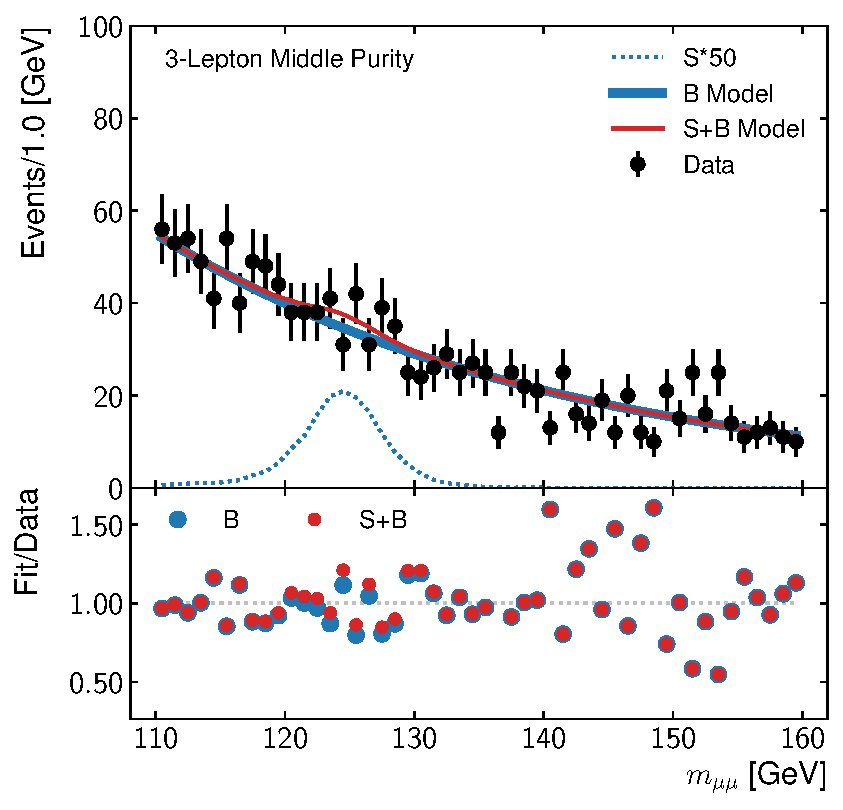
\includegraphics[width=0.5\textwidth]{figures/hmm/fitData/ratio-3lep1-dat.pdf}}}
\caption{Fits of the S+B and B-only models to the data observed in the exclusive 4-lepton high-purity (a), 3-lepton high-purity (b), and 3-lepton middle-purity categories.}
\label{fig:hmmPostcutFits}
\end{figure}


\subsection{Significance}

\begin{table}[htp]
\caption{Significance and p-values of the observed data yield in $\muu\in[120,130]$~GeV given the expected background.}
\begin{center}
\begin{tabular}{l r r r r r}\toprule
Category & Significance $\sigma$ & p-value \\
\midrule
3-lepton & 0.59 & 0.28 \\
4-lepton & 0.42 & 0.34 \\
\midrule
4-lepton High-Purity & 1.93 & 0.03 \\
3-lepton High-Purity & 0.84 & 0.20 \\
3-lepton Middle-Purity & 0.50 & 0.31 \\
\bottomrule\end{tabular} %remember cline{1-2}
\label{tab:hmmSignificance}
\end{center}
\end{table}

Table \ref{tab:hmmSignificance} presents the significances, given the background-only hypothesis, of each observation.
The top of the table shows these for the inclusive categories, while the bottom shows values for the exclusive categories.
These are separated to emphasize that the inclusive and exclusive category observations are correlated.
The largest significance is that of the observation in the 4-lepton High-Purity category, approaching 2$\sigma$.
The combined significance of the inclusive categories is 0.724$\sigma$.

The combined significance of the exclusive categories is $2.16\sigma$.
For comparison, the leptonic VH observation by CMS is cited with a significance of 2.02$\sigma$. \cite{cmsHmm}
This observation joins the ATLAS Run 2 measurements of VH, all of which have seen modest excesses beyond the Standard Model prediction. \cite{atlasHComb}

\subsection{Limits}

\begin{table}[htp]
\caption{Upper limits set at 95\% confidence levels on the signal strength \mus in each of the inclusive (top) and exclusive (bottom) categories. The signal strength corresponds to a number of signal events $N_S$, and these are provided as well.}
\begin{center}
\begin{tabular}{l r r r r r }
\toprule
\multirow{2}{*}{Category} & \multicolumn{2}{c}{Limit on $N_S$} & & \multicolumn{2}{c}{Limit on \mus} \\
\cline{2-3} \cline{5-6} 
& Expected & Observed & & Expected & Observed \\
\midrule
3-Lepton & 63.7 & 112.5 & &  13.2 & 22.6 \\
4-Lepton & 23.2 & 30.1 & &  33.2 & 42.8 \\
\midrule
4-Lepton High-Purity & 14.7 & 28.3 & &  23.7 & 45.1 \\
3-Lepton Middle-Purity & 58.1 & 94.4 & &  18.7 & 29.8 \\
3-Lepton High-Purity & 20.6 & 29.5 & &  12.0 & 17.2 \\
\bottomrule
\end{tabular}
\label{tab:hmmLimits}
\end{center}
\end{table}

None of the observations in Table \ref{tab:hmmSignificance} are significantly different from the background expectations.
Limits are consequently set on the production of Higgs-like signal events in the inclusive and exclusive categories.
The top half of Table \ref{tab:hmmLimits} reports limits set at 95\% confidence intervals for the inclusive categories.
These limits are set in the fiducial volume defined in Section \ref{sec:hmmEv}.
Fiducial volumes specify a multi-lepton phase space but do not make further requirements on the kinematic character of a potential signal.
This makes these limits relatively model-independent and interpretable in terms of other signal production mechanisms.
For this purpose, the limits are provided both on the signal strength \mus for the Standard Model VH, and in terms of the number of signal events $N_S$.
The bottom half of the table presents limits set at 95\% confidence intervals for the exclusive categories.
For these, the limits on the Standard Model signal strength are most relevant.
In all cases, the excesses reported in Table \ref{tab:hmmResultNdat} result in weaker observed limits than expected.

\subsection{\hmm Combination}

\subsection{Summary}

This chapter has presented a search for the Standard Model Higgs boson's rare decay to two muons (\hmm) using the VH production channels.
Detecting the decays of Higgs to two muons is particularly challenging on two counts.
First, the Higgs branching fraction to muons is tiny ($2.18\times10^{-4}$).
Second, there is a large irreducible dimuon background from Drell-Yan and Diboson processes.
A new strategy has been developed to use the leptonic final states of VH production to explore a new, unobserved phase space.
The additional leptons in these events help differentiate VH from the Drell-Yan background and provide kinematic information for further discrimination.

Studying VH/\hmm introduces additional challenges.
First is the tiny VH cross-section leading to relatively few signal events.
Second is how to use the new information from the W/Z leptonic decay products to separate the background from diboson production processes (ZZ and WZ).
% Techniques to address challenge
Detailed performance studies to develop a new set of selection criteria targeted at VH production to capture as many VH/\hmm events as possible.
Machine-learning methods in the form of a multivariate analysis discriminant were used to take advantage of the kinematic information from the W/Z decays.
Careful use of k-fold splitting and test/validation/train designations were introduced to avoid introducing uncontrolled bias.

No significant departure from the expected background is observed in data.
The limits set on signal production in the new phase spaces explored in this analysis are the first of their kind.
The strongest expected (observed) limit on leptonic VH production excludes signals down to 13.2(22.6) times the Standard Model prediction.
Limits are set on the numbers of signal events in 4-lepton and 3-lepton fiducial volumes.
These exclude the visible cross-section times branching ratio those regions above \xsbr=0.31~fb and \xsbr=0.16~fb respectively.
